%\documentclass{llncs}
\documentclass[journal, letterpaper]{IEEEtran}
%\documentclass{scrartcl}


\usepackage[ngerman,english]{babel}
%\usepackage[latin1]{inputenc}
\usepackage[utf8]{inputenc}
\usepackage[T1]{fontenc}
\usepackage{amsmath}
\usepackage{amsthm}
\usepackage{amsfonts}
\usepackage{tikz}
\usepackage{verbatim}
\usepackage{subcaption}
\usepackage{algorithm}
\usepackage{algorithmic}
\usepackage[pdftex]{hyperref}
\usepackage{graphicx}
\usepackage{caption}
\usepackage{subcaption}
\usepackage{listings}

\renewcommand{\algorithmicrequire}{\textbf{Input:}}
\renewcommand{\algorithmiccomment}[1]{\ \ // #1} % C-like // Comments
\lstset{language=Java, tabsize=4}

\hyphenation{render}

% No clubs and widows allowed
\clubpenalty10000
\widowpenalty10000
\displaywidowpenalty=10000

\begin{document}

%\title{Simulating elastic spheres without external forces}
%\subtitle{Project 1 for class CS6491 Computer Graphics}
\title{Procedural Terrain \\
	{\large Final project for class CS6491 Computer Graphics}}
%\author{Sebastian Weiss}
\author{Sebastian Weiss \\ \today}
%\date{\today}

\maketitle

\begin{tikzpicture}[remember picture,overlay]
   \node[anchor=north east,inner sep=0pt] at (current page.north east)
              {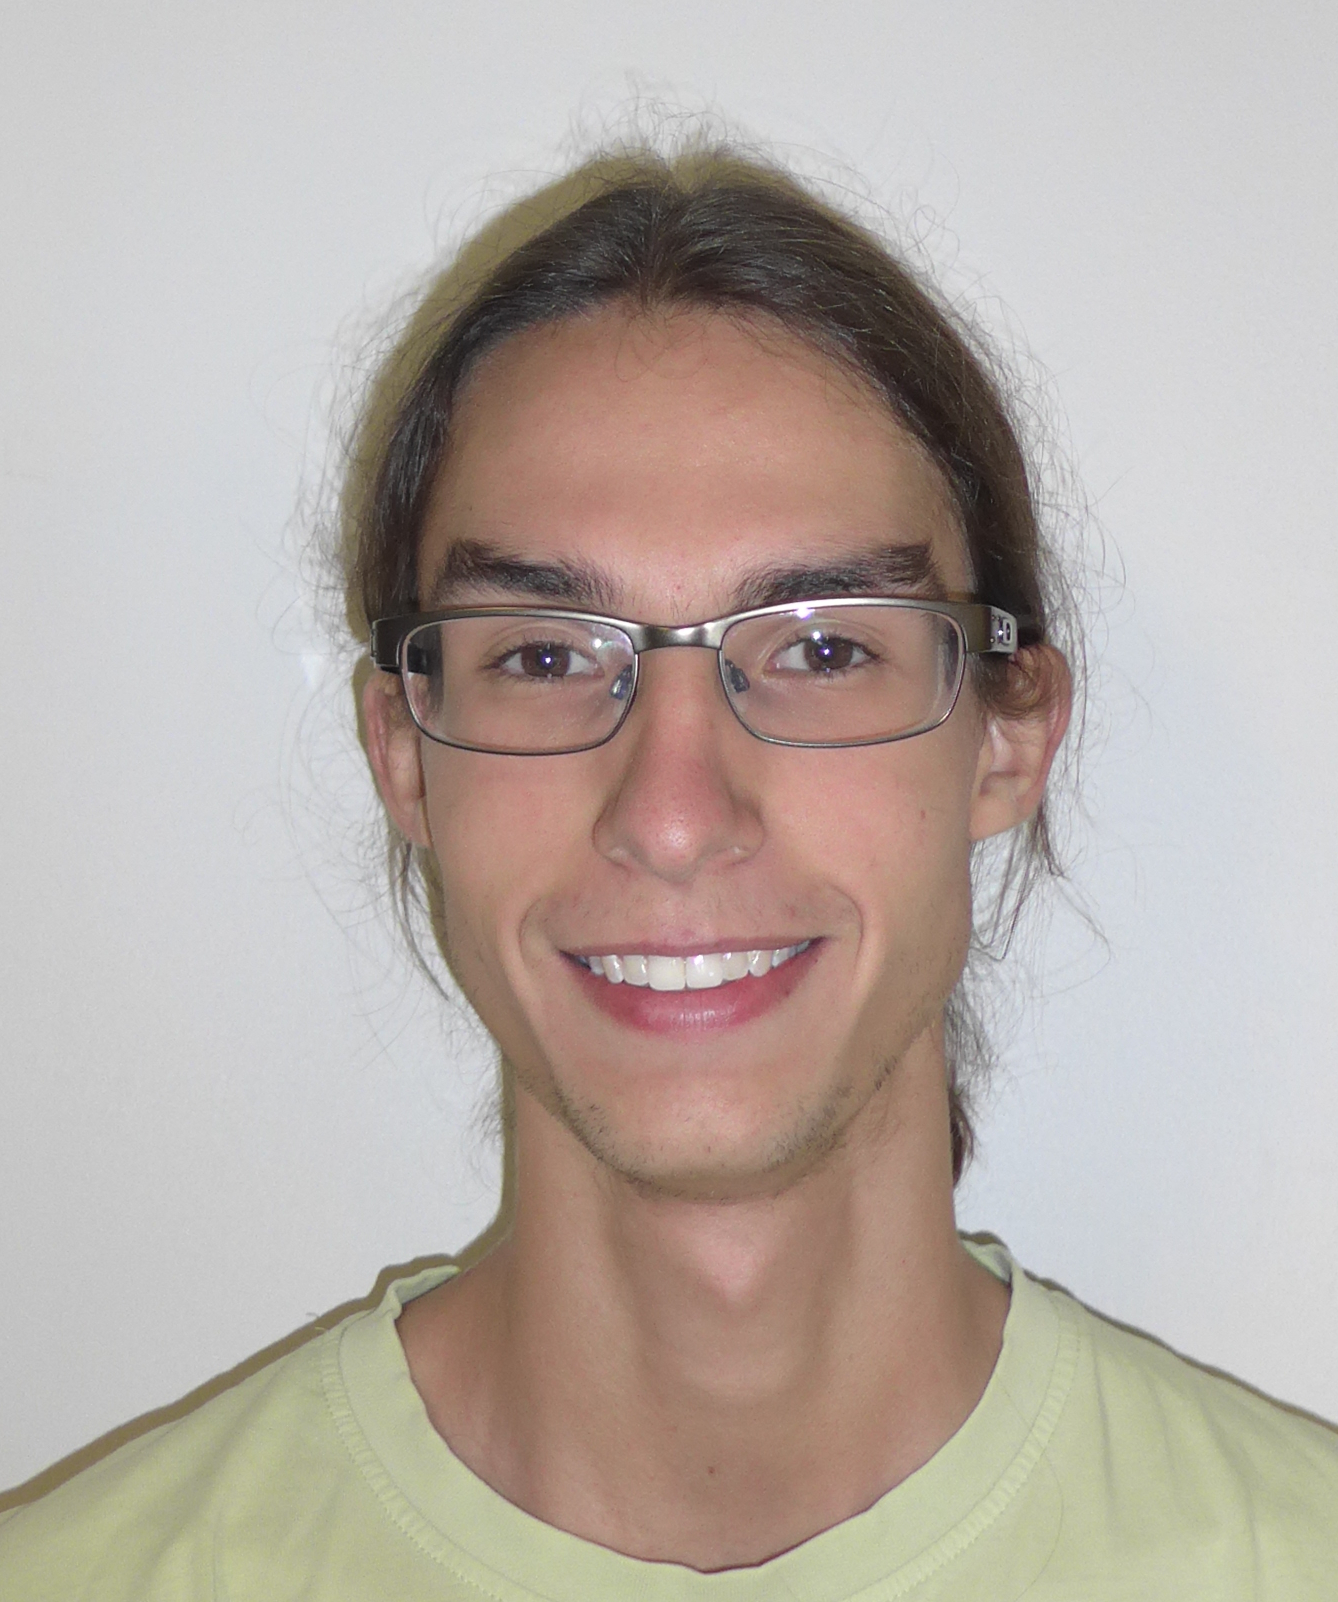
\includegraphics[scale=0.2]{pic}};
\end{tikzpicture}

\begin{abstract}
	Abstract
\end{abstract}

\section{Objective}
Terrain is a topic of endless discussion in computer graphics. It has to cover a large area of the world and at the same time it has to provide enough details for close-up shots.
It is extremely time consuming to create a large-scale terrain that is also interesting when viewed closely. 

In this project I present a framework for generating terrain, from a coarse grained height map to vegetation generation. The focus lies on combining existing techniques for performing the single tasks.
The result should be an island because it provides a natural border of the world.

Applications of procedural terrain include computer games, movies and geographic visualization and simulation.
The project was heavily inspired by a talk about "The Good Dinosaur" from Pixar Animation Studios.

\section{Related Work}
A lot of work has been done already in the field of generating height maps. There are in general three different approaches to this problem.
Generating the height map completely from scratch using perlin noise, fractals, voronoi regions, software agents or genetic algorithms are described in \cite{Doran.2010}, \cite{JacobOlsen.2004} and \cite{TeongJooOngRyanSaundersJohnKeyserJohnJ.Leggett.2005}. These models often lack realism because of the missing physically and geographic background. This is addressed in a second approach, hydraulic erosion models, as described in \cite{BedrichBenes.2007} and \cite{Mei.}. They start with existing height maps and increase the realism by simulating fluid to erode the terrain and forming rivers in the end. The other way is used in \cite{JeanDavidGenevauxEricGalinEricGuerinAdrienPeytavieBedrichBenes.2013}, here we start with a river network and build the terrain with respect to the river flow.
The last approaches copes with the lack of control in the previous described methods. They define the terrain by control features provided by the user, see \cite{FloraPonjouTasseArnaudEmilienMariePauleCaniStefanieHahmannAdrienBernhardt.2014} and \cite{Hnaidi.2010}.
On a 2D-scope, \cite{AmitPatel.2010} should be mentioned because it describes a complete new approach not using height map grids, but voronoi regions as base primitives.

After the terrain is created, it must be populated with vegetation. Rendering of grass is described in e.g. \cite{KurtPelzer.} and \cite{Boulanger.2005}. Trees must be generated first and for that, \cite{AdamRunionsBrendanLanePrzemyslawPrusinkiewicz.2007} and \cite{Weber.} should be mentioned.

\section{Overview}
The framework consists of the following steps that are executed one after another:
\begin{enumerate}
	\item generating an initial map using voronoi regions, chapter \ref{PolygonalMap}
	\item editing the terrain by user-defined features, chapter \ref{TerrainFeatures}
	\item simulate water and erosion to increase the realism, chapter \ref{HydraulicErosion}
	\item define biomes and populate the scene with grass and trees, chapter \ref{Vegetation}
\end{enumerate}

\section{Polygonal Map}\label{PolygonalMap}
As a first step, we have to come up with a good initial terrain to help the user with the terrain features.
These techniques are taken from \cite{AmitPatel.2010}.

\subsection{Voronoi Regions}
We could start with a regular grid of squares or hexagons, but using a Voronoi diagram provides more randomness.

At the beginning, we generate random points, called center points, in the plane from -1 to 1 in x and y coordinate and compute the Voronoi diagram (Fig. \ref{fig:voronoi}).

Because the shapes of the polygons are too irregular, we perform a relaxation step by replacing each center point by the average of the polygon corners (Fig. \ref{fig:relaxation}).
Applying this step several times results in more and more uniform polygons. In practice, two or three iterations provide good results.

\begin{figure*}
	\centering
	\begin{subfigure}[b]{0.3\textwidth}
		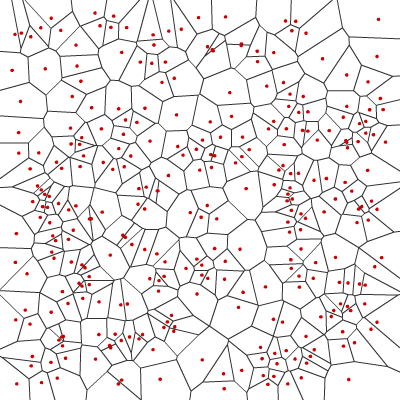
\includegraphics[width=\textwidth]{images/voronoi-polygons}
		\caption{initial region}
		\label{fig:voronoi}
	\end{subfigure}
	\begin{subfigure}[b]{0.3\textwidth}
		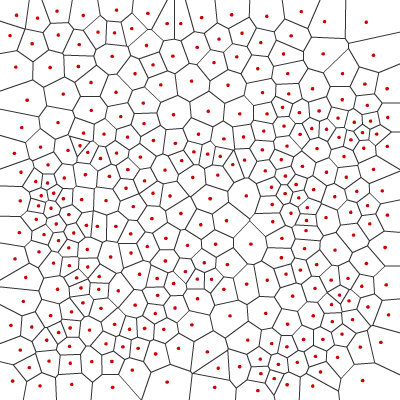
\includegraphics[width=\textwidth]{images/voronoi-2-lloyd}
		\caption{relaxation}
		\label{fig:relaxation}
	\end{subfigure}
	\begin{subfigure}[b]{0.3\textwidth}
		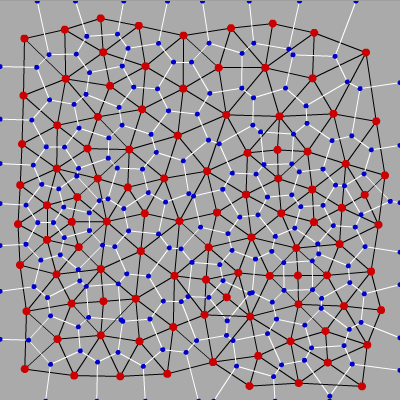
\includegraphics[width=\textwidth]{images/voronoi-and-delaunay}
		\caption{graph representation}
		\label{fig:graph}
	\end{subfigure}
	\caption{Initial polygon map}\label{fig:PolygonalMap}
\end{figure*}

\subsection{Graph representation}
For further processing of the polygons, we have to build a graph representation (Fig. \ref{fig:graph}).
The graph datastructure consists of the following three classes:
\begin{lstlisting}
	class Center  {
		int index;
		Vector2f location;
		boolean water;
		boolean ocean;
		boolean border;
		Biome biome;
		float elevation;
		float moisture;
		float temperature;
		List<Center> neighbors;
		List<Edge> borders;
		List<Corner> corners;
	}
\end{lstlisting}
\begin{lstlisting}
	class Edge {
		int index;
		Center d0, d1; //Delaunay
		Corner v0, v1; //Voronoi
		Vector2f midpoint;
		int riverVolume;
	}
\end{lstlisting}
\begin{lstlisting}
	class Corner {
		int index;
		Vector2f point;
		boolean ocean;
		boolean water;
		boolean coast;
		boolean border;
		float elevation;
		float moisture;
		float temperature;
		int river;
		List<Center> touches;
		List<Edge> incident;
		List<Corner> adjacent;
	}
\end{lstlisting}
The class Center stores the center of a voronoi region, and the vertices of the voronoi polygons are represented by Corner. Because of the duality between the Voronoi Diagram and Delaunay triangulations, an edge connects both two corners (as an edge of a voronoi polygon) and two centers (as an edge in the delaunay triangulations).
The other properties of the three classes are needed in the next step.

\subsection{Island shape}
As a next step, we have to define the general shape of the island.
A simple way to get the desired shape is to combine perlin noise\footnote{http://mrl.nyu.edu/~perlin/doc/oscar.html} with a distance from the center.
Let $(x,y)$ be a point and we want to know if it is in the water or not.
\begin{equation}
 noise := \sum_{i=0}^n{\text{noise}(x\: o_b\: o_s^i, y\: o_b\: o_s^i)\:a_b\: a_s^{-i}}
\label{eq:elevation1}
\end{equation}
\begin{equation}
	water(x,y) := noise < offset + scale\:(x^2,y^2)
\label{eq:elevation2}
\end{equation}
The function $water(x,y)$ returns true iff the point $(x,y)$ is in the water. The function noise(x,y) returns the value of the perlin noise at the specified position.

There are many values to tweak: $n$ defines the number of octaves that are summed together, $o_b$ specifies the base octave, $o_s$ the octave scale, $a_b$ the base amplitude and $a_s$ the amplitude scale. $scale$ defines the influence of the distance to the center of the map versus the perlin noise and $offset$ is the specifies a base island size.
In our experiments, we use the following values: $n=4, o_b=6, o_s=2, a_b=0.5, a_s=2.5, scale=2.2, offset=-0.2$.

This function is evaluated for every corner (stored in the water-property). A center is labeled as water if at least 30\% of the corners are water.
The result can be seen in Fig. \ref{fig:shape}

\begin{figure*}
	\centering
	\begin{subfigure}[b]{0.3\textwidth}
		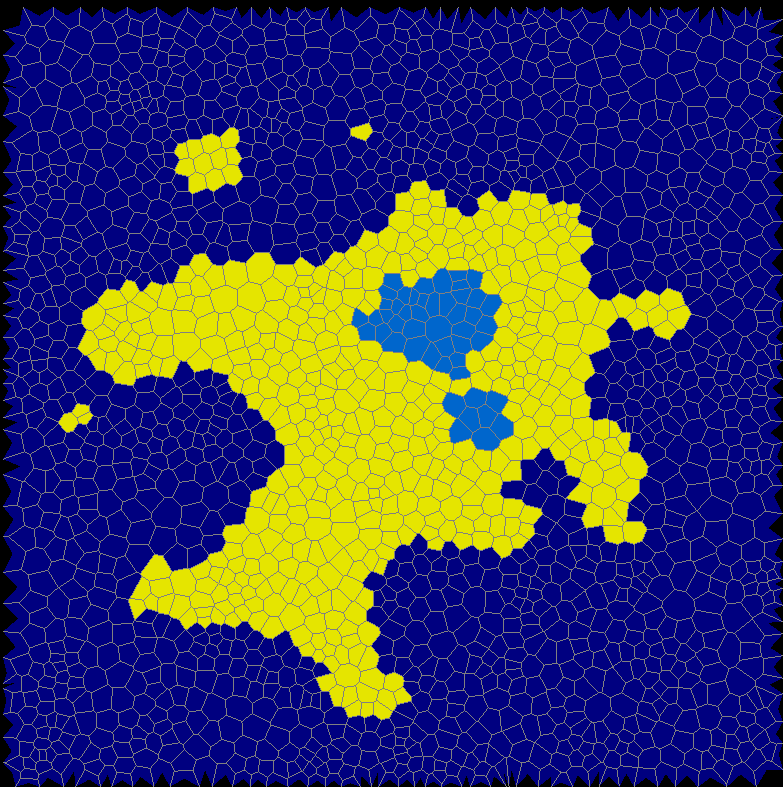
\includegraphics[width=\textwidth]{images/elevation1}
		\caption{initial shape}
		\label{fig:shape}
	\end{subfigure}
	\begin{subfigure}[b]{0.3\textwidth}
		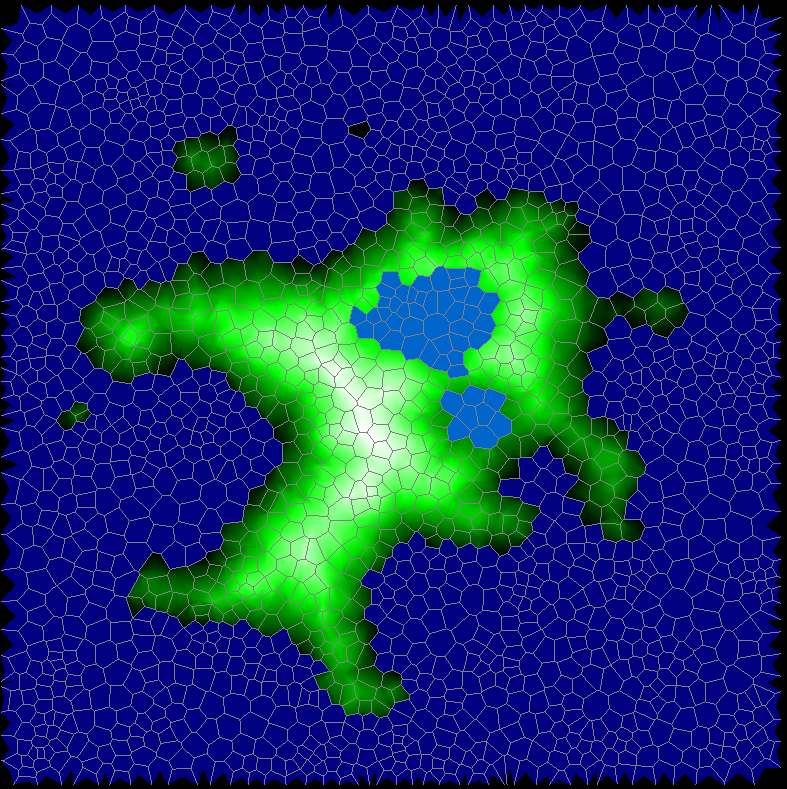
\includegraphics[width=\textwidth]{images/elevation2}
		\caption{elevation}
		\label{fig:elevation}
	\end{subfigure}
	\begin{subfigure}[b]{0.3\textwidth}
		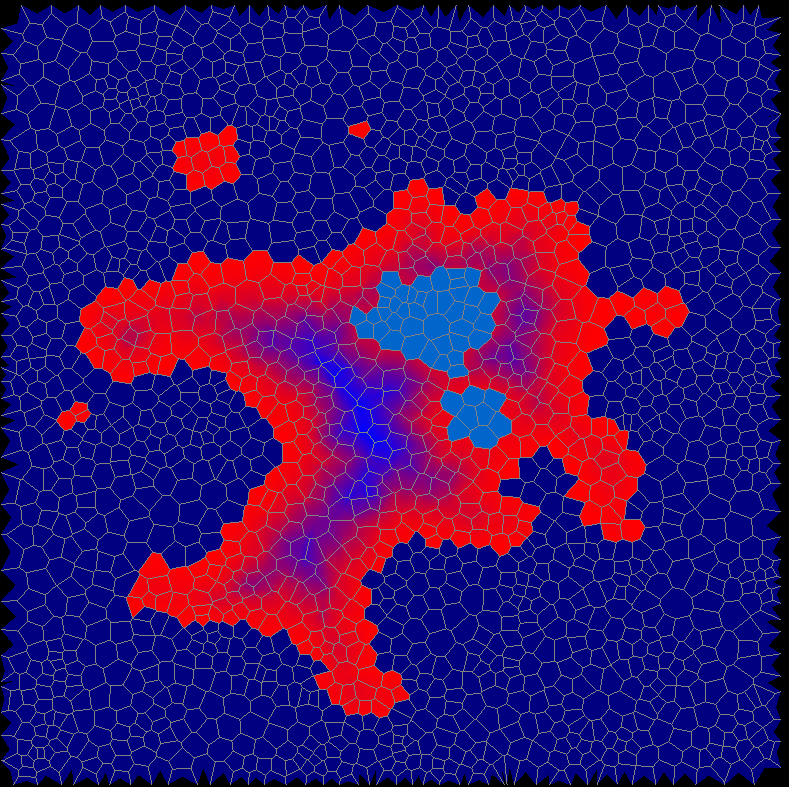
\includegraphics[width=\textwidth]{images/temperature}
		\caption{temperature}
		\label{fig:temperature}
	\end{subfigure}
	\begin{subfigure}[b]{0.3\textwidth}
		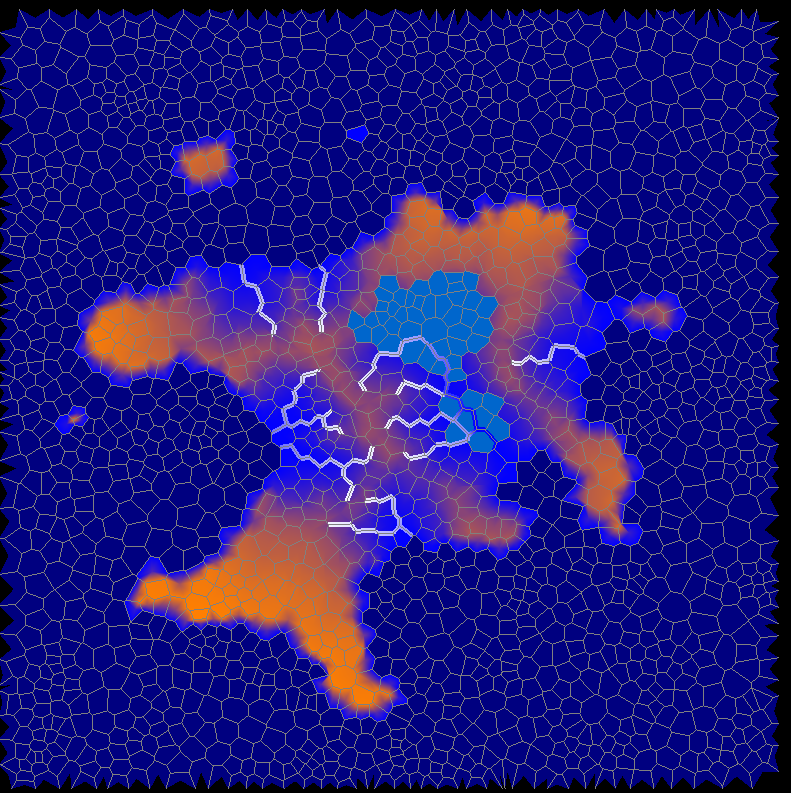
\includegraphics[width=\textwidth]{images/moisture}
		\caption{moisture}
		\label{fig:moisture}
	\end{subfigure}
	\begin{subfigure}[b]{0.3\textwidth}
		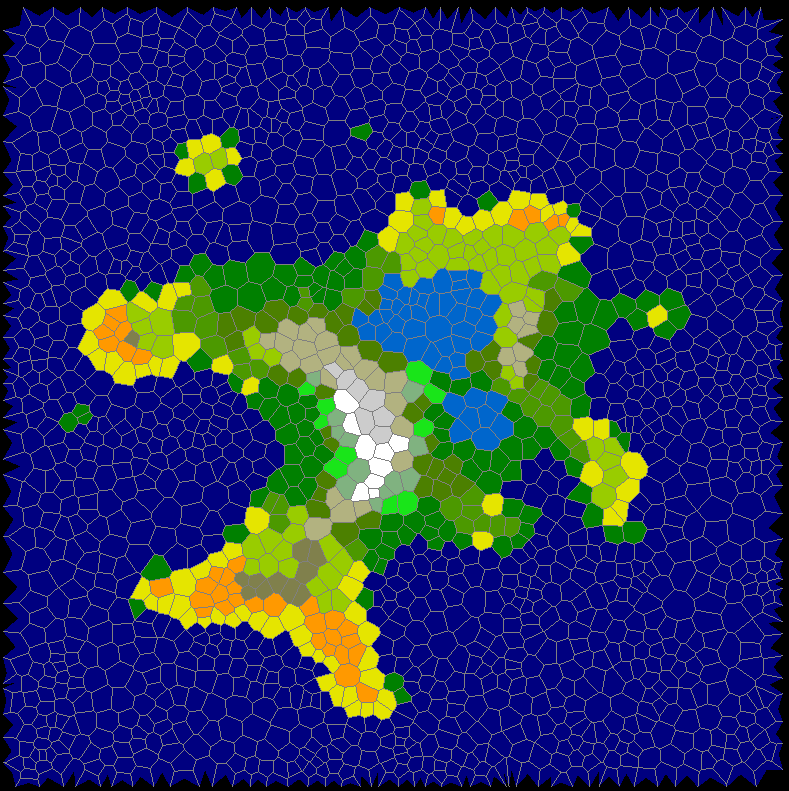
\includegraphics[width=\textwidth]{images/biomes}
		\caption{biomes}
		\label{fig:biomes}
	\end{subfigure}
	\begin{subfigure}[b]{0.3\textwidth}
		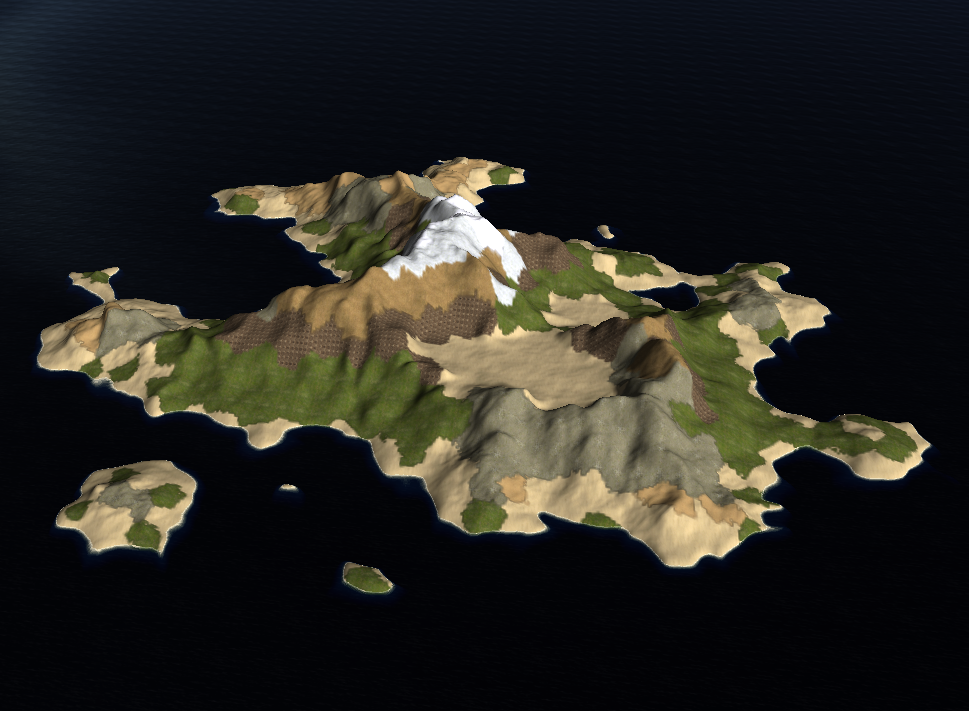
\includegraphics[width=\textwidth]{images/heightmap}
		\caption{generated heightmap}
		\label{fig:heightmap}
	\end{subfigure}
	\caption{Elevation and Moisture}\label{fig:PolygonalMap2}
\end{figure*}

To distinguish between oceans and lakes, we use a flood fill from the border of the map and mark every water polygon on the way as 'ocean' until we reach the coast.
Corners are marked as 'coast' if they touch centers that are ocean and land.

\subsection{Elevation}\label{Elevation}
After creating the initial island shape, we assign elevation values to every corner and center (Fig. \ref{fig:elevation}).
For that we start from every coast corner and traverse the graph using breath-first along the corners. When traversing over land, we increase the elevation and over the sea we decrease the elevation. By that we obtain mountains and a continental shelf. Only when walking along or over lakes, we do not increase the elevation. This leads to flat areas that are later filled with water.

From the elevation, we directly derive the temperature: The higher it is, the colder it is. (Fig. \ref{fig:temperature}).

Until now, the elevation and temperature were defined for corners. To get these values for centers as well, we simply average them.

\subsection{Moisture}\label{PolygonalMoisture}
To obtain moisture values, we start with creating rivers.

First we select random corners that are not coast or water and from there we follow the path of the steepest descent until reaching the ocean. At each step, we increase the amount of water the river carries. We then initial the moisture value of the river corners with the water amount. To achieve more distributed rivers, you might start a new river only at corners that are at least one or two steps away from an existing river.

Second we perform a breath-first-search starting from river corners. At each step, we decrease the moisture by a multiplicative factor of e.g. 0.8 (works well in our experiments). By that, the rivers spread their moisture over the land depending on the amount of water they carry.

Third we average again the moisture of each corner to obtain the moisture per center.
The result can be seen in \ref{fig:moisture}.

As a last step, we assign a biome to each center based on its temperature and moisture (Fig. \ref{fig:biomes}). This acts as a starting point for chapter \ref{Vegetation}. More details on the biomes are described in section \ref{Biomes}.

\subsection{Generating the height map}
\subsubsection{Heightmap}
The next steps in the processing pipeline all require a heightmap. A height map is just a rectangular grid of values where each cell stores the height at this point. We also use the same datastructure to store moisture and temperature values.

Notation: Let $H$ be the heightmap. Then we identified the cell at position $i,j$ with either $H_{i,j}$ or $H[i,j]$, depending on the readability. When coordinates lie outside the map, we clamp them. When the coordinates are not integers, but lie between cells, we perform a bilinear interpolation between the neighboring cells. When two heightmaps, or in the general case two scalar- or vectorfields, are added or multiplied together in this paper, these are always element-wise operations.

\subsubsection{Base elevation}
Since we already display the polygon graph from the previous steps using triangle meshes, we can just render the elevation mesh from step \ref{Elevation} to obtain a base elevation of the generated terrain. 

However, the straight corners of the polygonal cells are still visible. Therefore we have to distort the height map by replacing each height with the height of the cell an offset away. The offset is defined by a perlin noise. For more details on this, see chapter "Combination and perturbation" in \cite{JacobOlsen.2004}. The increase the height difference between flatlands and mountains, we apply the following scaling to the height values:
\begin{equation}
	h \leftarrow sign(h) \cdot |h|^{1.5}
\label{eq:HeightScaling}
\end{equation}

\subsubsection{Adding noise}
The terrain still looks very boring, we need more noise to create hills and mountains.
Therefore we add a multi fractal noise to the heightmap. The equation is taken from Chapter 4.3 of \cite{Hnaidi.2010}.
\begin{equation}
	N(x,y) := A(x,y) \sum_{k=0}^n \frac{\text{noise}(r^k x, r^k y)}{r^{k(1-R(x,y)}}
\label{eq:HeightmapNoise}
\end{equation}
noise is again the perlin noise function, $r$ is the octave factor (here $r=2$) and $n$ is the number of octaves (we use $n=5$). The scalarfield $A$ defines the amplitude of the noise at the given terrain position and $R$ the roughness (how the octaves are mixed together).
In our experience we compute $A$ and $R$ based on the biomes using the values from table \ref{tab:NoiseProperties}.
\begin{table}[htbp]
	\centering
		\begin{tabular}{l|c|c}
			Biome & $A$ & $R$ \\ \hline
			Snow & 0.5 & 0.7 \\
			Tundra & 0.5 & 0.5 \\
			Bare & 0.4 & 0.4 \\
			Scorched & 0.7 & 0.3 \\
			Taiga & 0.4 & 0.3 \\
			Shrubland & 0.5 & 0.2 \\
			Temperate desert & 0.1 & 0.1 \\
			Temperate rain forest & 0.3 & 0.2 \\
			Deciduous forest & 0.3 & 0.4 \\
			Grassland & 0.4 & 0.5 \\
			Tropical rain forest & 0.3 & 0.2 \\
			Tropical seasonal forest & 0.3 & 0.2 \\
			Subtropical desert & 0.3 & 0.6 \\
			Beach & 0.3 & 0.5 \\
			Lake & 0.2 & 0.2 \\
			Ocean & 0.2 & 0.1
		\end{tabular}
	\caption{Noise properties}
	\label{tab:NoiseProperties}
\end{table}
The noise value $N$ is then simply added to the final height map.

The result can be seen in Fig. \ref{fig:heightmap}. (The seed used is 658175619cff )

\subsection{User interaction}
In our implementation, the user can modify the elevation, temperature and moisture values starting from the presented initial values.
By that, the user can create custom island shapes, raise mountains, build valleys and define the biomes by editing the temperature and moisture values.

With the terrain created in this step, we can proceed to the next step.

\section{Terrain Features}\label{TerrainFeatures}
Starting from the terrain from the previous chapter, the user has now the ability to fine-tune the terrain features.
This is an implementation of \cite{Hnaidi.2010} with some extensions. More examples and further explanations are available in this paper.

\begin{figure*}
	\centering
	\begin{subfigure}[b]{0.45\textwidth}
		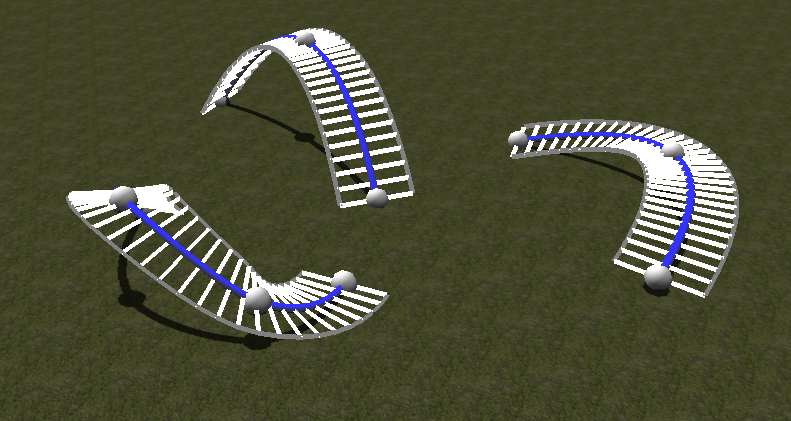
\includegraphics[width=\textwidth]{images/diffusion1}
		\caption{feature curves}
		\label{fig:featurecurves}
	\end{subfigure}
	\begin{subfigure}[b]{0.45\textwidth}
		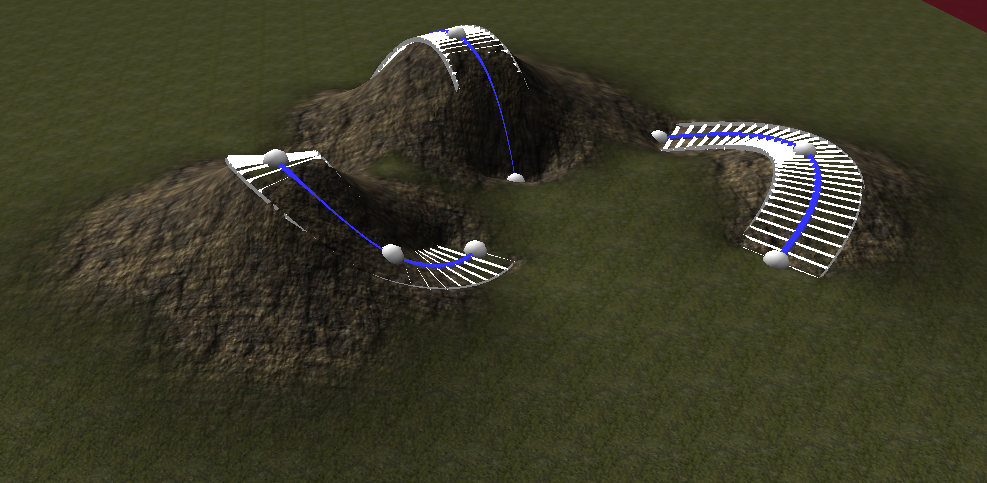
\includegraphics[width=\textwidth]{images/diffusion2}
		\caption{resulting terrain}
		\label{fig:resultingterrain}
	\end{subfigure}
	\caption{Defining feature curves}\label{fig:diffusion1}
\end{figure*}
\subsection{Feature curves}
In the center of this processing steps stand feature curves. Feature curves are added by the user and a solver (\ref{DiffusionSolver}) then modifies the terrain with respect to them.
Example feature curves forming hills can be seen in Fig. \ref{fig:featurecurves} (white spheres are the control points and the blue tupe is the interpolated curve) and the resulting terrain in Fig. \ref{fig:resultingterrain}.

Each feature curve consists of two or more control points. Each control point has the following properties:
\begin{itemize}
	\item a position $(x,y,z)$ in the world
	\item a boolean if it constraints elevation
	\item a float $plateau$, specifying the size of the flat plateau on top of the curve
	\item four floats $s_l, \varphi_l, s_r, \varphi_r$ specifying the size and angle of the slopes left and right of the curve
\end{itemize}
In the example in Fig. \ref{fig:diffusion1}, the slope sizes are zero, so no slope constraints are applied.

Between the control points, the position is interpolated using cubic hermit splines and quadratic hermit splines at the start and end point (I use the code from the CurveAverage project).
The other constraining values are linearly interpolated. 

\subsection{Diffusion solver}\label{DiffusionSolver}
The task of the diffusion solver is to modify the terrain so that it remains smooth while preserving the feature constraints.
The diffusion solver iteratively updates the terrain using the following recursion: Let $H^i$ be the height map at the i-th iteration.
\begin{equation}
\begin{array}{rcl}
	H^{k+1}[i,j] &=& \alpha[i,j] E[i,j]  \\
	             &+& \beta[i,j] G^{k+1}[i,j]  \\
							 &+& (1-\alpha[i,j]-\beta[i,j]) L^{k+1}[i,j]
\end{array}
\label{eq:Diffusion1}
\end{equation}
$E$ is the forced elevation at the given point, it is directly created from the elevation constraints of the feature curves.
$G$ describes the gradient or the slope and $L$ is a Laplace smoothing term.
The values $\alpha$ and $\beta$, with $0\leq\alpha\leq 1, 0\leq\beta\leq 1, \alpha+\beta\leq 1$, specify the weighting of the single term. On the plateaus of the feature curves we set $\alpha=0.9$ and $\beta=0$. This forces the elevation to match the desired height while adding a little bit of smoothing to it. During slopes of the feature curve, we use $\alpha=0$ and $\beta=0.5$. By that, both the slope constraints and smoothing constraints are satisfied. Outside of the influence of the feature curves, we set $\alpha=0, \beta=0$.

The gradient term is defined in the following way:
\begin{equation}
	G^{k+1}[i,j] = N^k[i,j]+G[i,j] \newline
\label{eq:Diffusion2}
\end{equation}
\begin{equation}
	N^k[i,j] = \textbf{n}_x^2 H^k[i-\text{sign}(\textbf{n}_x),j] + \textbf{n}_y^2 H^k[i, j-\text{sign}(\textbf{n}_y)]
\label{eq:Diffusion3}
\end{equation}
The gradient equation tend to satisfy the provided gradient $G$. $G$ is directly calculated from $\sin(\varphi_l)$ and $\sin(\varphi_r)$, i.e. from the slope angles defined at the control points.
The vector $\textbf{n}=(\textbf{n}_x,\textbf{n}_y)$ describes the normalized direction of the gradient. This vector is orthogonal to the feature curve when projected in the plane and point away from the curve. In Fig. \ref{fig:featsExist2}, some of them are displayed as gray lines going away from the plateau.

The Laplace term smoothes the terrain by averaging the neighbor cells:
\begin{equation}
\begin{array}{rcl}
	L^{k+1}[i,j] &=& \frac{1}{4}(H^k[i-1,j]+H^k[i+1,j] \\
							 & & +H^k[i,j-1]+H^k[i,j+1])
\end{array}
\label{eq:Diffusion4}
\end{equation}

\begin{figure*}
	\centering
	\begin{subfigure}[b]{0.3\textwidth}
		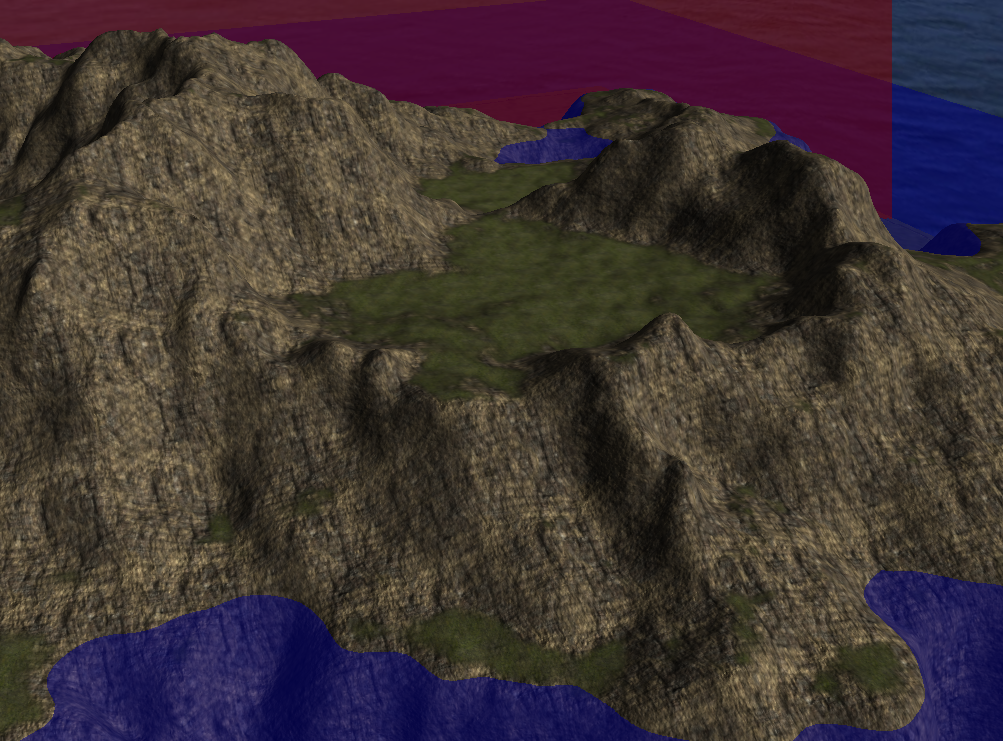
\includegraphics[width=\textwidth]{images/diffusionEditExisting1}
		\caption{original terrain}
		\label{fig:featsExist1}
	\end{subfigure}
	\begin{subfigure}[b]{0.3\textwidth}
		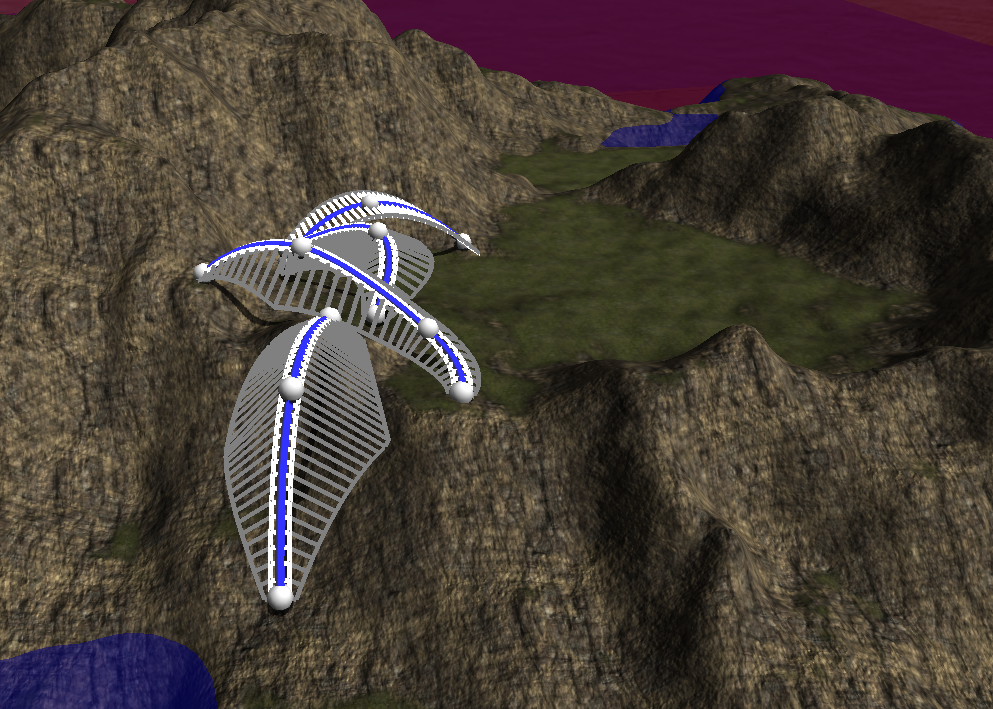
\includegraphics[width=\textwidth]{images/diffusionEditExisting2}
		\caption{adding feature curves}
		\label{fig:featsExist2}
	\end{subfigure}
	\begin{subfigure}[b]{0.3\textwidth}
		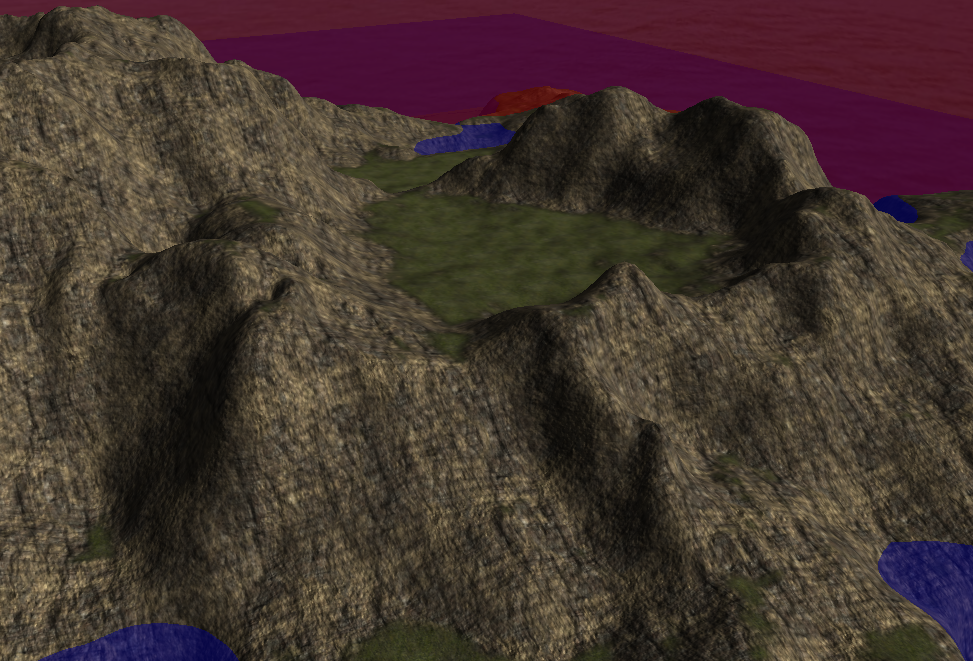
\includegraphics[width=\textwidth]{images/diffusionEditExisting3}
		\caption{resulting terrain}
		\label{fig:featsExist3}
	\end{subfigure}
	\caption{Adding features to existing terrain}\label{fig:diffusion2}
\end{figure*}
\subsection{Integrate into existing terrain}
Defining the whole terrain only with the feature curves is very tedious. Therefore we want to start with an existing terrain, as described in chapter \ref{PolygonalMap}.
However, simply starting with the existing terrain as $H^0$ does not work because the Laplace term would just smooth out every feature apart from the feature curves.

\cite{FloraPonjouTasseArnaudEmilienMariePauleCaniStefanieHahmannAdrienBernhardt.2014} proposes a different solution. They compute the elevation and gradient constraints relative to the original terrain, then solve the diffusion equation on a flat map and add them together. The idea is visualized in the following image:
\begin{center}
	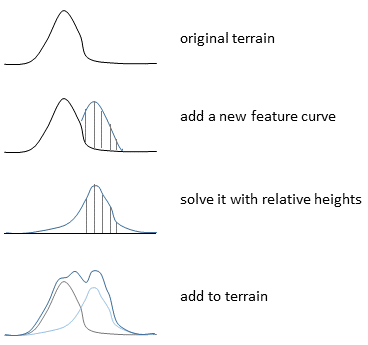
\includegraphics[width=0.30\textwidth]{images/DiffusionAddFeatures}
\end{center}
This works as long as there are no sharp features already existing right next to the new feature curve. If that is the case, as in the image above, adding the curves together produces unwanted results because of these inferences.

This case happens quite often as seen in Fig. \ref{fig:diffusion3}. Here we define a new feature curve right next to an existing mountain. Although the curve's slope does not touch the existing terrain, the smoothing term inside the diffusion solver also increases the height outside of the feature curve. This leads to a growth of the mountain on the left (the tip of the mountain is now much higher than the control point, before it was about the same height).
From a designer's perspective, this behavior might be not wanted because it is hard to predict and control.

\begin{figure*}
	\centering
	\begin{subfigure}[b]{0.3\textwidth}
		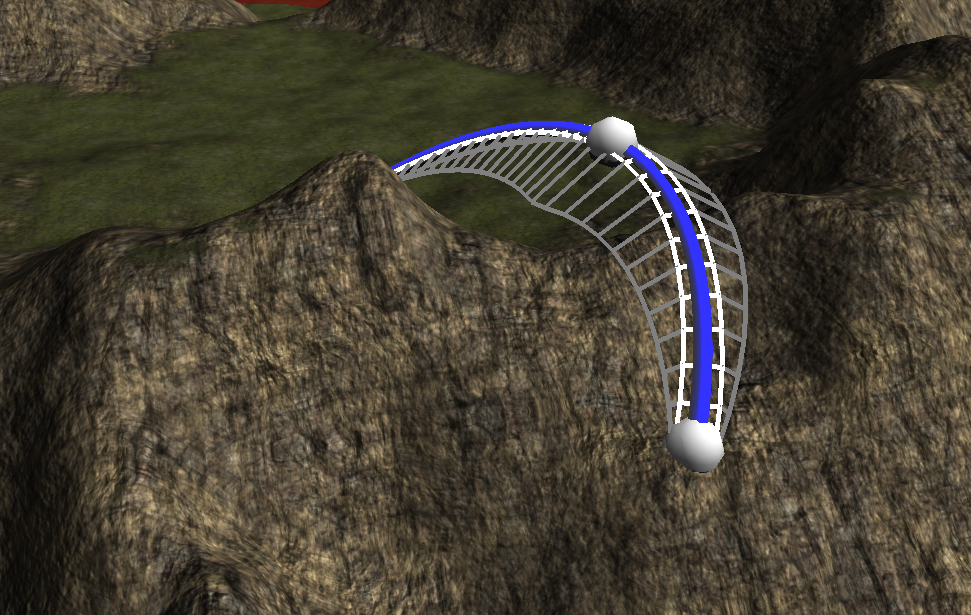
\includegraphics[width=\textwidth]{images/diffusionError1}
		\caption{original terrain with new feature curve}
		\label{fig:diffusionError1}
	\end{subfigure}
	\begin{subfigure}[b]{0.3\textwidth}
		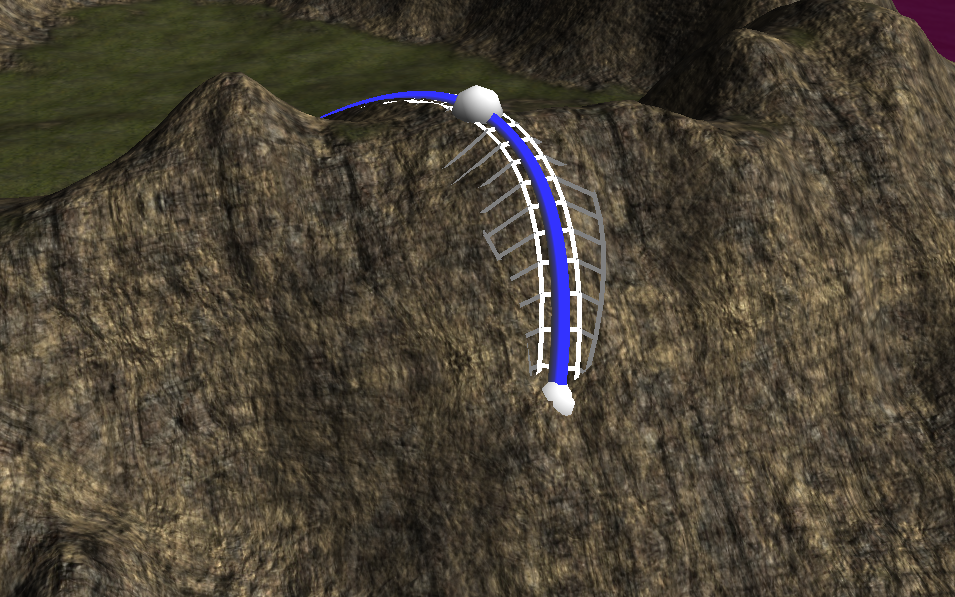
\includegraphics[width=\textwidth]{images/diffusionError2}
		\caption{inference, left mountain is modified}
		\label{fig:diffusionError2}
	\end{subfigure}
	\begin{subfigure}[b]{0.3\textwidth}
		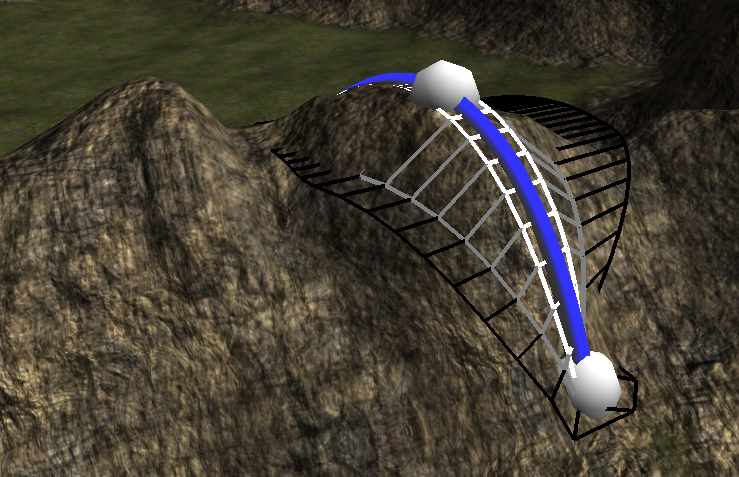
\includegraphics[width=\textwidth]{images/diffusionErrorSolved}
		\caption{limiting smoothing to remove inference}
		\label{fig:diffusionError3}
	\end{subfigure}
	\caption{Inferences between new feature curves and existing terrain features}\label{fig:diffusion3}
\end{figure*}

\subsection{Extension of the solver}
We propose now another solution that both keeps existing terrain features while it preserves the local control and removes the inferences mentioned before.
The idea is to limit the smoothing term $L$ to influence only a customizable region around a feature curve.
For this, we add two new parameters, $l_l$ and $l_r$, to each control point. They specify the local radius of an envelope around the plateau and slope of the feature curve.
It not only extends along the slope, but also over the start and end of the feature curve. 

We then set $\gamma$ to 1 inside this envelope and to 0 outside and modify equation \ref{eq:Diffusion1} to include $\gamma$:
\begin{equation}
\begin{array}{rcl}
	H^{k+1}[i,j] &=& \alpha[i,j] E[i,j]  \\
	             &+& \beta[i,j] G^{k+1}[i,j]  \\
							 &+& \gamma[i,j] (1-\alpha[i,j]-\beta[i,j]) L^{k+1}[i,j]
\end{array}
\label{eq:Diffusion1_mod}
\end{equation}

Because we no limit the smoothing area, we can apply the solver directly on the original height map without smoothing out existing features. There is no need anymore to solve the diffusion equation on a separate map with relative heights as done in the previous section.

In Fig. \ref{fig:diffusionError3} you see the problematic situation again, but this time, the smoothing region is bounded as described before. The border of the smoothing envelope is visualized by the black lines. Note that the old mountain is preserved and the new feature is blended into the terrain without discontinuities.

\section{Hydraulic Erosion}\label{HydraulicErosion}
Now the shape of the terrain is fully defined, and the next step is to increase the realism by performing erosion.

Erosion is comes in many shapes in the nature: there is thermal erosion which decomposes larger stones into smaller ones, wind erosion which carries sand over long distances and finally water erosion.
Water erosion or hydraulic erosion is caused by flowing water that erodes the terrain, transports sediment along the river and finally deposits it somewhere.
Since the hydraulic erosion is the strongest one, we focus on this type of erosion in the presented framework.

We use an adapted version of the model presented in \cite{Mei.}.

\subsection{Erosion Model}
The algorithms follows the following steps, which are repeatedly executed using the timestep $\Delta t$ (e.g. $\Delta t = 0.01$):
\begin{enumerate}
	\item increment water by rainfall
	\item flow simulation
	\item change water volume
	\item erosion, deposition and sediment transportation
	\item evaporation
\end{enumerate}
In the next sections, we use the following notation for describing the involved variables, all of them are scalarfields or vectorfields on the grid of the terrain:
\begin{itemize}
	\item terrain height $b$
	\item water height $d$
	\item suspended sediment $s$
	\item outflow flux $\textbf{f}=(f^L,f^R,f^T,f^B)$
	\item water velocity $\textbf{v}=(u,v)$
\end{itemize}
\begin{center}
	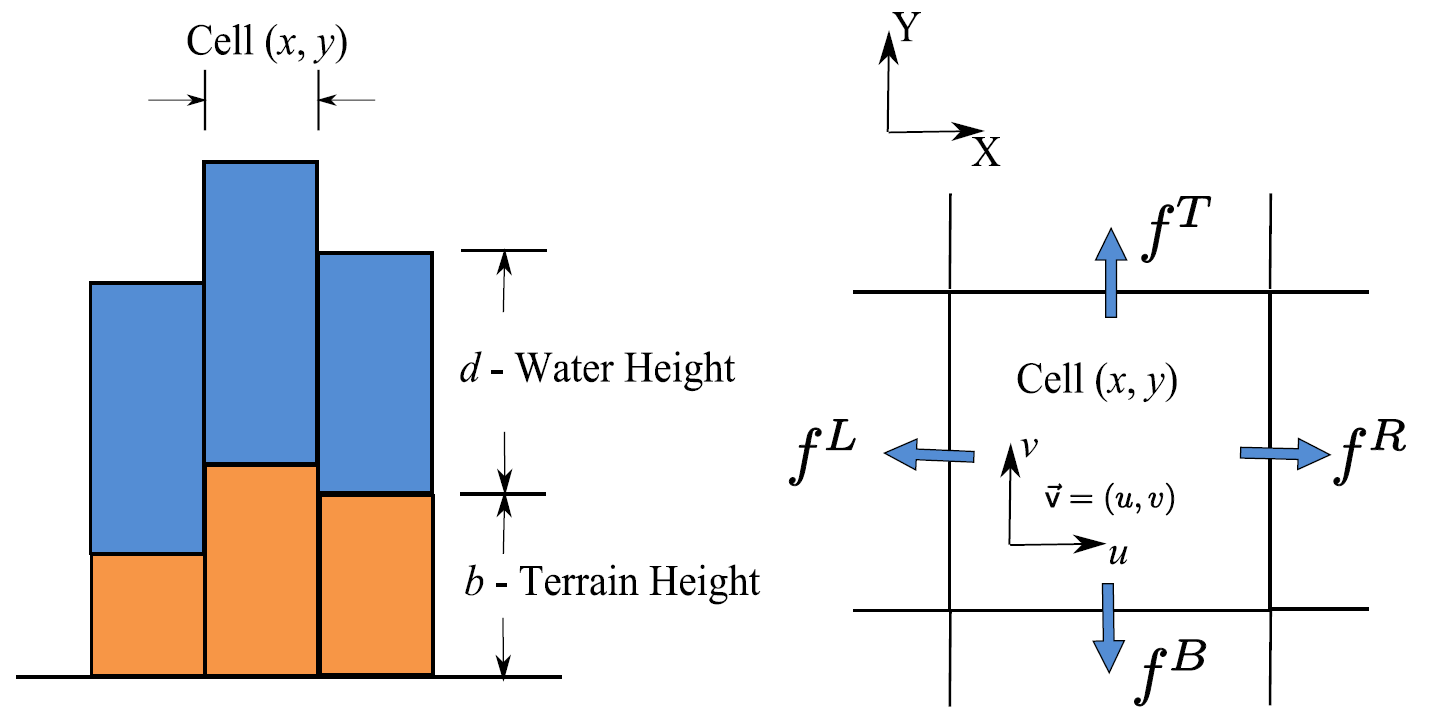
\includegraphics[width=0.4\textwidth]{images/erosionVariables}
\end{center}

\subsubsection{Water increment}
Rainfall is simulated by sampling water drops over the terrain. The probability of each cell to 'emit' a water drop is equal to the moisture. The moisture map is initialized with the information created at the very beginning, in chapter \ref{PolygonalMoisture}. The user can edit this moisture value before starting the simulation. By using random rain drops instead of a global water increment, we add more randomness to the scene. A single raindrop erodes the terrain a little bit, forming a tiny river bed. Next drops that are created nearby are now more likely to follow this path as well. This then leads to formation of river beds instead of just removing sediment from slopes uniformly.

In addition, the user can place river sources on the terrain. They act as a constant source of water.

Let $r_t[x,y]$ be the water that arrives at the current time step at position $(x,y)$. Then the water height is modified in the following way:
\begin{equation}
	d_t[x,y] = d_t[x,y] + \Delta t \cdot r_t[x,y]
\label{eq:ErosionRain}
\end{equation}

\subsubsection{Flow simulation}
In the flow simulation, we simulate the way water flows from higher positions to lower positions. We approximate this by using virtual pipes that connect two adjacent cells in the grid. The amount of water that flows from one cell to the other is called the outflow flux.

The outflow flux from the current cell to the neighbor cell to the left is computed as follows:
\begin{equation}
	f_{t+\Delta t}^L[x,y] = \max(0, f_t^L[x,y]+\Delta t \cdot g \cdot \Delta h_t^L[x,y]
\label{eq:ErosionFlow1}
\end{equation}
Whereby the height difference to the left cell is calculated using:
\begin{equation}
	\Delta h_t^L[x,y] = b_t[x,y]+d_t[x,y]-b_t[x-1,y]-d_t[x-1,y]
\label{eq:ErosionFlow2}
\end{equation}
$f^R$, $f^T$ and $f^B$ are calculated in the same way.
The gravitation constant $g$ specifies the amount of acceleration of the flow by the height difference. In our experiments, we set $g=10$.

It can now happen that after subtracting the sum of the outflow flux from the water height (see \ref{Erosion3}), the water height becomes negative.
To avoid this, all four outflow flux values are scaled with the following scaling factor $K$ (evaluated cell-wise).
\begin{equation}
	K=\min(1, \frac{d}{(f^L+f^R+f^T+f^B)\cdot \Delta t})
\label{eq:ErosionFlow3}
\end{equation}

\subsubsection{Water volume change}\label{Erosion3}
After computing the outflow flux, we can define the change of the water volume as:
\begin{equation}
\begin{array}{rcl}
	\Delta V[x,y] &=& \Delta t \cdot (\sum{f_{in}} - \sum{f_{out}}) \\
	              &=& \Delta t \cdot (f_{t+\Delta t}^L[x+1,y] + f_{t+\Delta t}^R[x-1,y] \\
								& & f_{t+\Delta t}^B[x,y+1] + f_{t+\Delta t}^T[x,y-1] \\
								& & - \sum_{i\in\{L,R,T,B\}}{f_{t+\Delta t}^i[x,y]} )
\end{array}
\label{eq:ErosionVolume1}
\end{equation}
The water height per cell is then modified using:
\begin{equation}
	d_{t+\Delta t}[x,y] = d_t[x,y] + \Delta V[x,y]
\label{eq:ErosionVolume2}
\end{equation}
For the next step, \ref{ErosionDeposition}, we need to compute the horizontal velocity of the water $\textbf{v}=(u,v)$.
Let $\bar{d}$ be the arithmetic average of the water height before and after equation \ref{eq:ErosionVolume2}.
Then the velocity along the x-axis is compute as:
\begin{equation}
	u = \frac{f^R[x-1,y]-f^L[x,y] + f^R[x,y]-f^L[x+1,y]}{2\bar{d}}
\label{eq:ErosionVolume3}
\end{equation}
$v$, the velocity along the y-axis is computed similarly.

\subsubsection{Erosion, deposition and sediment transportation}\label{ErosionDeposition}


\subsection{Adaptions and limitations}

\section{Vegetation}\label{Vegetation}
TODO
\subsection{Biomes}\label{Biomes}

\section{Conclusion and future work}
TODO

\bibliographystyle{IEEEtran}
%\bibliographystyle{alpha}
\bibliography{Paper}
\end{document}